
Consider the function $$f(x_1,x_2)=2x_1^2+3x_2^2+x_1-x_2+3$$ illustrated in the figures below.

\begin{center}
  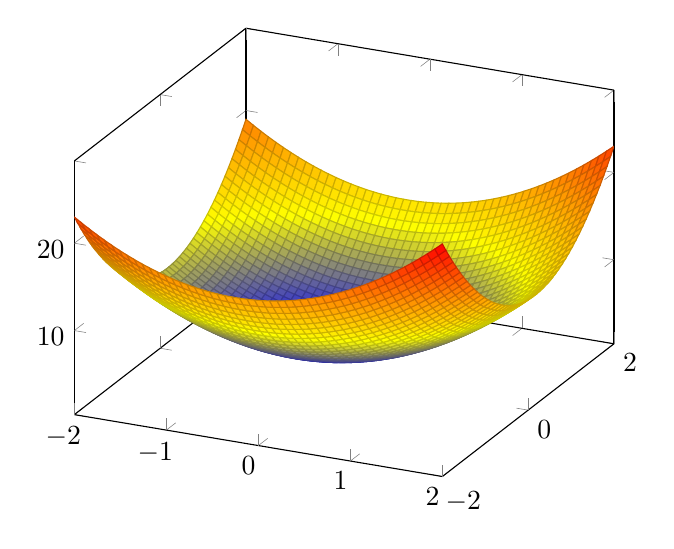
\begin{tikzpicture}
      \begin{axis}
     \addplot3[surf,domain=-2:2,samples=50]
      {2*x^2+3*y^2+x-y+3};
      \end{axis}
   \end{tikzpicture}
\end{center}


\begin{center}
  \begin{tikzpicture}
      \begin{axis}[view={0}{90},domain=-2:2]
     \addplot3[contour gnuplot={labels=false,number=40,handler/.style=smooth},samples=101]
      {2*x^2+3*y^2+x-y+3};
      \end{axis}
   \end{tikzpicture}
\end{center}

Show that
\[
x^*=\cvect{-\frac{1}{4} \\\frac{1}{6}}
\]
is a global minimum of $f$. Is it the only one?




